\subsection{The Renewable Energy Transition}\label{sec:external-energy_transition}


\subsubsection{Definition}

The term "energy transition" refers to the current global shift from fossil fuels to renewable energy sources to meet the urgent need to reduce greenhouse gas emissions, combat climate change, and enhance energy security. This transition encompasses a fundamental transformation of energy supply and consumption patterns, including the increased use of sustainable energy to achieve a low-carbon economy. Historical shifts in energy sources—from biomass to coal, and later to oil and natural gas—reflect the ongoing evolution of energy use. The present focus is on scaling up renewables such as solar and wind, which are becoming increasingly cost-competitive. Key aspects of the transition include adopting electric vehicles, improving public transportation, advancing energy-efficient technologies for building heating, and developing energy storage and grid solutions to support the integration of variable renewable energy sources.

\subsubsection{Future energy mix in the EU}

The projected electricity mix for the EU is presented in \autoref{fig:energy_mix}. An interactive figure can be viewed \href{https://futuram-project.github.io/FutuRaM.github.io/WP2/assets.html}{here~\faLink}

\begin{figure}[h!]
    \centering
    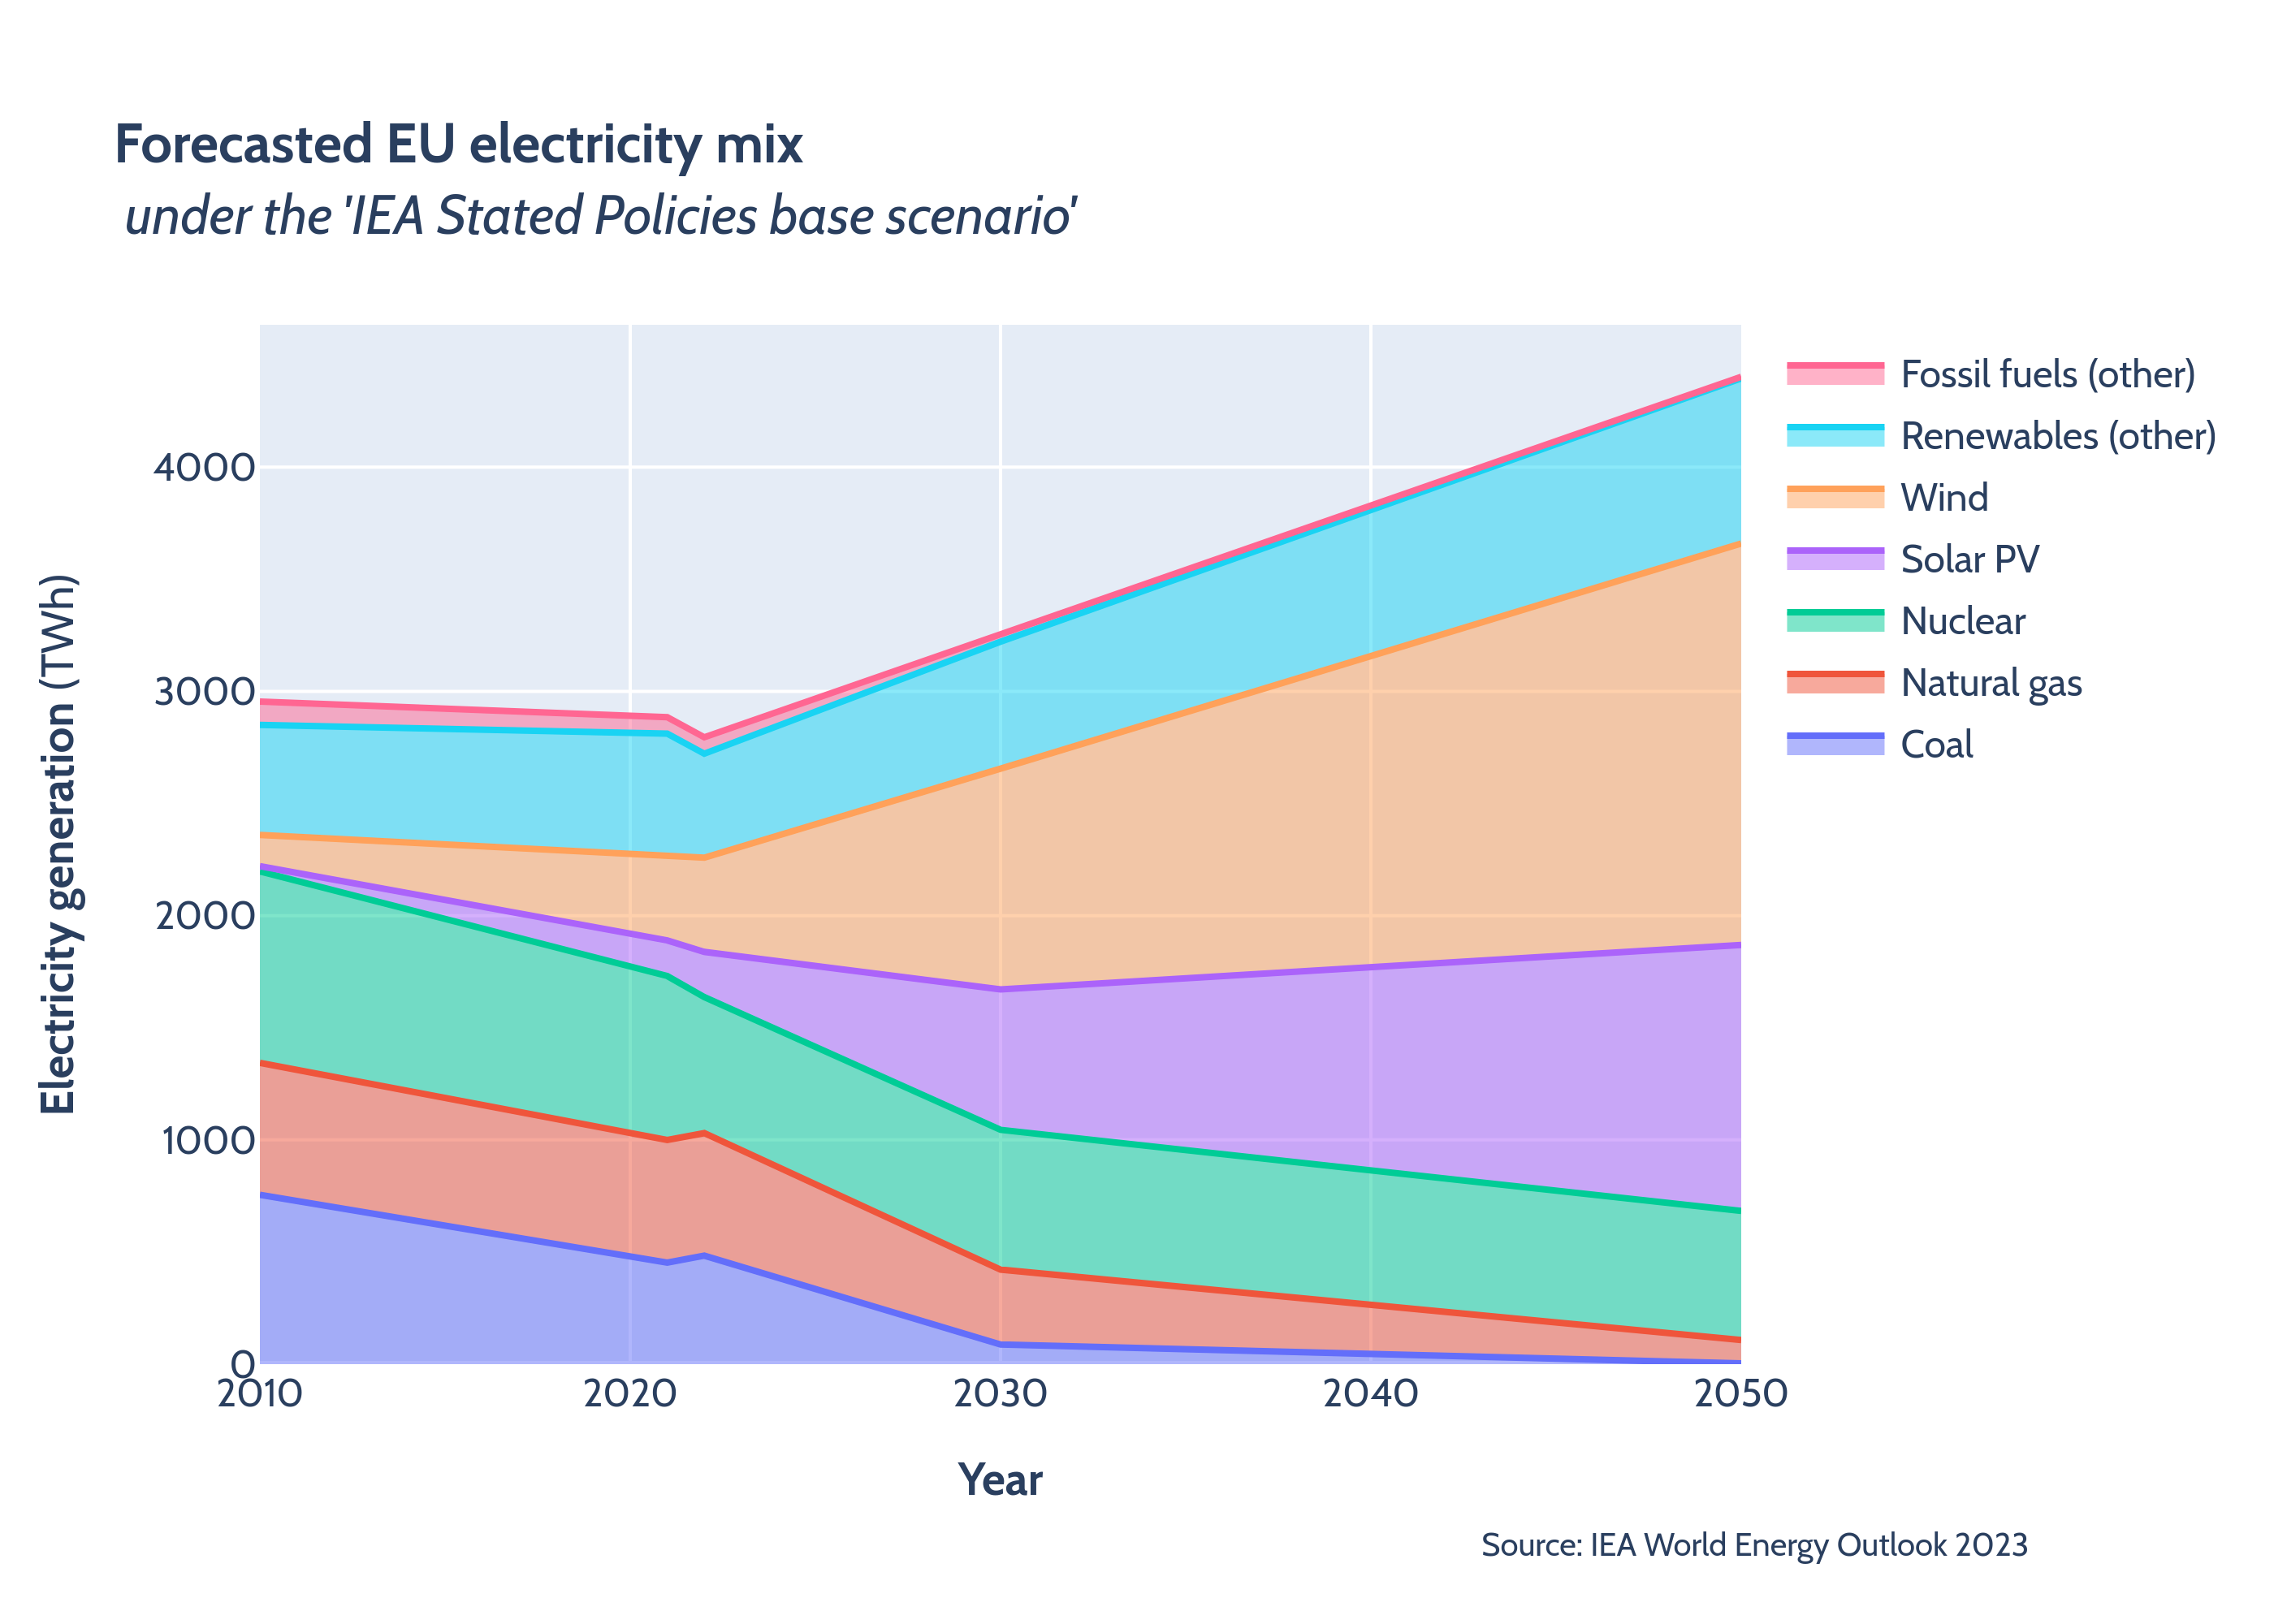
\includegraphics[width=\textwidth]{130quantification/external/energy_mix_forecast.png}
    \caption{EU electricity mix forecast until 2050}\label{fig:energy_mix}
\end{figure}

\subsubsection{Brief context of renewable energy in the EU}

Renewable energy is integral to the EU's shift towards a low-carbon economy and reducing reliance on imported fossil fuels—a response accentuated by the urgency to curtail dependence on Russian energy sources. The EU's strategic move is encapsulated in the REPowerEU Plan of Action, introduced in May 2022, and agreed upon in 2023 which prescribes an aggressive uptake of renewables, emphasizing wind and solar PV, alongside hydrogen, heat pumps, and batteries, vital for energy storage and transportation decarbonisation \cite{jrc2023supplychain,eu2023energy,eu2022repower, jrc2022energyclimateoutlook}.

In analysing the renewable sector in FutuRaM, the focus is on solar PV, wind turbines, electrolysers, batteries, and residential heat pumps. Other renewable sources like bioenergy, hydro, geothermal, and ocean energy, while part of the portfolio, are expected to have minimal impact on critical materials demand and are not central to this analysis.

\subsubsection{Justification for setting as an external scenario factor}

The ongoing global energy transition is a profound shift that holds implications for almost every facet of society, especially regarding CRMs, other raw materials and the system of waste management. This transition from fossil fuels towards renewable energy sources demands a significant increase in various CRMs, influencing their supply and demand curves extensively. In the development of FutuRaM's scenarios, the energy transition is recognised as a fundamental driver of change. However, for the purposes of focussed and strategic scenario modelling, it has been categorised as an external factor.

This classification allows for a delineation between direct policy levers within the purview of SRM systems and broader macro-environmental trends that, while influential, are not the primary subject of analysis within FutuRaM. As such, the project's scenarios incorporate a consistent baseline projection of the energy transition's effects, shared across the three scenarios, ensuring that the core analysis remains centred on material-centric policy outcomes and targets of the CRM act. This ensures that the resulting insights are actionable and tailored to the nuances of material management and recycling systems. It reflects a strategic choice to maintain scenario tractability and avoid the dilution of policy implications that could arise from an overly broad scope of variables.

Moreover, the scenario architecture within FutuRaM is constructed with inherent flexibility, permitting later incorporation of amendments to the background energy transition trends. This adaptability is essential to ensure that, as the energy landscape evolves and new data becomes available, the scenarios can be revised and updated, thereby preserving the relevance and accuracy of the project's findings over time.


\subsubsection{Relevant technologies in the renewable energy sector}

The cornerstone technologies in renewable energy—batteries, electrolysers, wind turbines, heat pumps, and solar PV—play pivotal roles across various sectors (Figure 85). Heat pumps serve industrial processes, while solar PV and batteries support ICT, defence, and mobility with energy and uninterrupted power supplies, respectively \cite{jrc2023supplychain}.

Wind energy, expected to surge, will benefit from cost-efficient, innovative turbines designed for increased productivity in offshore and low-wind conditions. Projections from GECO present two scenarios: a conservative estimate shows wind capacity expanding from 732 GW (2020) to 1,400 GW (2030), and to 4,050 GW by 2050. An optimistic forecast anticipates a rise to 2,500 GW by 2030 and 8,400 GW by 2050.

Solar PV is poised for exponential growth due to advancements enhancing efficiency and lowering costs. GECO's cautious scenario predicts growth from 710 GW (2020) to 2,950 GW (2030), reaching 7,500 GW by 2050. The optimistic scenario projects a tenfold increase by 2030 and sixteenfold by 2050 compared to 2020 levels.

Addressing the intermittency of wind and solar power necessitates adequate storage solutions and robust grid systems, with electrolysers emerging as a crucial technology for renewable hydrogen production, forecasted to exceed 1 GW capacity by the end of 2022 \cite{iea2022renewables}.

Additionally, digitalisation, robotics, and 3D printing are set to boost the renewable sector's productivity and optimisation across its value chain. Heat pump sales are also on an upward trend, with a peak expected in 2045, ranging between 15 million (low demand) and 38 million units (high demand) by 2050.

Material demand in the renewable sector is dominated by wind turbines, electrolysers, and solar PV, with wind energy leading in consumption of critical materials.


\subsubsection{Supply Chain bottlenecks in renewable energy}

Supply chain bottlenecks present a significant challenge in the deployment of renewable energy technologies, particularly for wind turbines, solar PV, electrolysers, and heat pumps. The production of NdFeB permanent magnets for wind turbines demands rare earth elements (REEs) like neodymium, dysprosium, praseodymium, and terbium, with the EU being highly dependent on imports for both raw and processed materials such as permanent magnet alloys and components like blades.

Solar PV technologies necessitate strategic raw materials, including silicon metal and rare metals like gallium and germanium, with China dominating the production of silicon ingots and wafers. This reliance on imports extends across the value chain, including the crystalline silicon cell production where the EU's contribution is minimal.

The battery industry utilizes strategic raw materials such as lithium, manganese, and cobalt, with raw materials and components largely imported. A shift is anticipated towards nickel-rich batteries or alternative chemistries to reduce reliance on high-cobalt-content lithium-ion batteries (LIBs) due to the oligopoly control of critical components in Asia.

Electrolysers for hydrogen production use a range of strategic raw materials, particularly from the platinum group metals (PGMs), but also silicon metal, aluminium, copper, and magnesium, with the EU facing challenges in sourcing these materials. For heat pumps, strategic raw materials needed include magnesium and copper, but no significant bottlenecks have been identified, with most critical materials used in microchips and IT controllers.

Across all technologies analysed, a common pattern of heavy reliance on imports, particularly from China, is observed at different stages of the value chains. The EU’s primary sourcing and processing capabilities for critical raw materials are notably low, creating dependencies at multiple levels. Despite a strong manufacturing capacity for wind turbine assembly, the EU is entirely reliant on imports for the value chain of rare-earth permanent magnets. Similarly, for solar PV, the dependence on imports is comprehensive. The recent surge in Chinese manufacturing market share for heat pumps and the developing value chain for batteries in the EU are also noteworthy.

A breakdown of the materials required for each technology is given in \autoref{tab:energy-crms}.


\newgeometry{left=2cm,right=2cm,top=2cm,bottom=2cm}
\begin{landscape}
    \centering
    \small
    \renewcommand{\arraystretch}{0.8} % adjust the value as needed
    \begin{longtable}{|C{2cm}|L{3cm}|C{2cm}|C{2cm}|C{2cm}|C{2cm}|C{2cm}|C{2cm}|}
        \caption{Raw materials essential to the renewable energy sector}\label{tab:energy-crms}\\
        \hline
        \rowcolor{headerblue} % Applying the header color
        \color{white}\textbf{SUPPLY RISK} & \color{white}\textbf{MATERIAL} & \color{white}\textbf{CRM} & \color{white}\textbf{BATT} & \color{white}\textbf{H2} & \color{white}\textbf{WIND} & \color{white}\textbf{SOLAR (PV)} & \color{white}\textbf{HEAT PUMPS} \\
        \hline
        \endfirsthead%
        \hline
        \multicolumn{8}{r}{\textcolor{headerblue}{\textit{{Continued on next page}}}}\\
        \endfoot%
        \rowcolor{white}
        \multicolumn{8}{c}{{\textcolor{headerblue}{\textit{\tablename\ \thetable{} --- Continued from previous page}}}}\\
        \hline
        \rowcolor{headerblue} % Applying the header color
        \color{white}\textbf{SUPPLY RISK} & \color{white}\textbf{MATERIAL} & \color{white}\textbf{CRM} & \color{white}\textbf{BATT} & \color{white}\textbf{H2} & \color{white}\textbf{WIND} & \color{white}\textbf{SOLAR (PV)} & \color{white}\textbf{HEAT PUMPS} \\
        \endhead%
        \bottomrule
        \endlastfoot%
        \csvreader[separator=comma, late after line=\\]{csvs/energy-crms.csv}{}{
            \csvcoli & \csvcolii & \csvcoliii & \csvcoliv & \csvcolv & \csvcolvi & \csvcolvii & \csvcolviii
        }
    \end{longtable}
    \renewcommand{\arraystretch}{1} % reset \arraystretch to its original value
    \end{landscape}
\restoregeometry% restore margins to normal


The integration of the energy transition has significant implications for the management of Critical Raw Materials (CRMs) across various waste streams due to changing material requirements and waste profiles~\cite{jrc2023supplychain,jrc2020reedemanddata,iea2023energytechperspectives,iea2023crm}.

\vspace{\baselineskip}
\textbf{For example:}

\wasteSubsubsubsecBATT
\vspace{-1cm}
\begin{itemize}
    \item Increased deployment of Li-ion batteries for energy storage will lead to a surge in waste batteries, necessitating improved recycling technologies to recover CRMs.
    \item The transition to renewable energy sources may lead to changes in the battery composition, affecting recycling processes and the types of CRMs that need to be managed.
\end{itemize}

\wasteSubsubsubsecELV
\vspace{-1cm}
\begin{itemize}
    \item The shift towards electric vehicles will transform the composition of ELVs, increasing the relevance of CRMs used in electric powertrains and batteries.
    \item This transition requires the adaptation of ELV recycling infrastructure to efficiently process and recover new types of CRMs.
\end{itemize}

\wasteSubsubsubsecWEEE
\vspace{-1cm}
\begin{itemize}
    \item As energy systems become more digitized and interconnected, WEEE will contain a broader array of CRMs, prompting the need for more sophisticated recycling methods.
    \item The growing volume of WEEE will challenge current recycling capacity and technology, calling for significant innovation in CRM recovery techniques.
\end{itemize}

\wasteSubsubsubsecCDW
\vspace{-1cm}
\begin{itemize}
    \item Green building materials and energy-efficient technologies may introduce new CRMs into CDW, changing the material recovery landscape.
    \item The promotion of deconstruction over demolition could preserve the integrity of materials containing CRMs, allowing for better recovery rates.
\end{itemize}

\wasteSubsubsubsecMIN
\vspace{-1cm}
\begin{itemize}
    \item The drive for clean energy technologies is expected to increase the mining of specific CRMs, potentially leading to higher volumes of mining waste that must be managed sustainably.
\end{itemize}

\wasteSubsubsubsecSLASH
\vspace{-1cm}
\begin{itemize}
    \item The energy transition could increase the generation of certain industrial wastes such as slags, which may contain valuable CRMs.
\end{itemize}

\vspace{\baselineskip}
\subsubsection{Implementation in EU Law}

\subsubsubsection{Fit for 55 Package (2021)}

The "Fit for 55" package is a collection of policy initiatives proposed by the European Commission in July 2021 aimed at revising and updating EU legislation to reflect the increased ambition of reducing net greenhouse gas emissions by at least 55\% by 2030, compared to 1990 levels~\cite{eu2021fitfor55}. This target was a significant step up from the previous goal of a 40\% reduction and is part of the European Union's plan to become climate-neutral by 2050 --- an objective set out in the European Green Deal\cite{eu2019greendeal}.

The package includes proposals to revise the EU Emissions Trading System (ETS), to increase the use of renewable energy, to improve energy efficiency, and to implement carbon pricing mechanisms, among other measures. The intention is to align existing laws with the 2030 climate target and to set the legal foundation for Europe's transition to a green economy. This includes changes across various sectors including transportation, building, and energy production to reduce emissions and promote sustainable practices.

\subsubsubsection{REPowerEU Plan (2022)}

The invasion of Ukraine by Russia has caused significant disruption to energy markets in Europe and globally. To eliminate reliance on an unreliable supplier, the European Commission has devised the REPowerEU plan~\cite{eu2022repower}. This initiative focuses on energy conservation, the production of clean energy, and the diversification of energy sources, supported by financial and legal measures to develop Europe's necessary new energy infrastructure and systems.

\paragraph{Accelerating Clean Energy} Renewable energy sources, being both cost-effective and environmentally friendly, can be produced locally, thereby reducing dependency on imported energy. The REPowerEU plan aims to expedite the green transition and trigger substantial investments in renewable energy. It also seeks to facilitate the rapid transition of industry and transport from fossil fuels, reducing both emissions and dependency.

This includes a variety of measures focused on renewable energy and energy efficiency, such as:

\begin{itemize}
    \item Increasing the EU's 2030 renewable energy target of the `Fit for 55 package' from 40\% to 45\%.
    \item Accelerating the deployment of photovoltaic (PV) energy.
    \item Introducing the European Solar Rooftop Initiative.
    \item Doubling the deployment rate of individual heat pumps.
    \item Decarbonising the industry by promoting electrification and renewable hydrogen.
    \item Speeding up renewable energy project and grid infrastructure permit processes.
    \item Increasing the EU’s binding energy savings target for 2030 to 13\%.
\end{itemize}

The May 2022 REPowerEU plan by the European Commission, in response to the energy market disruptions due to Russia's invasion of Ukraine, is designed to rapidly cut down on the EU's reliance on Russian fossil fuels. It raises the renewable energy target of the Fit for 55 package from 40\% to 45\%.

This ambitious goal for renewable energy use, coupled with REPowerEU’s strategies to reduce energy demand, necessitates substantial increases in renewable capacity across the electricity, transport, and heating and cooling sectors. The Commission forecasts that to meet the 2030 objectives, renewable electricity should reach 69\%, 32\% in transport, and a yearly growth of at least 2.3 percentage points in heating and cooling.


\subsubsubsection{Renewables Energy Directive (2023)}

The recent legislation strengthening the EU Renewable Energy Directive marks an advancement towards the European Green Deal and REPowerEU ambitions. With the provisional agreement, the EU's binding renewable energy target for 2030 is now at least 42.5\%, aiming potentially to reach 45\%. This target significantly surpasses the previous goal of 32\% and is nearly double the present proportion of EU renewable energy.

A distinct enhancement over the REPowerEU plan is the establishment of definitive binding targets for renewable energy. The legislation optimises permitting procedures, acknowledges renewable energy as an overriding public interest, and designates acceleration zones for expedited development in strategically identified regions.

The directive also introduces specific directives across various sectors:

\begin{itemize}
    \item In heating and cooling, it sets forth progressive annual renewable targets and a 49\% renewable energy consumption benchmark in buildings by 2030.
    \item It for the first time includes the industrial sector under its ambit, establishing indicative and binding targets for the use of renewable energy and renewable hydrogen, respectively.
    \item For the transport sector, it specifies a reduction in greenhouse gas intensity and sets sub-targets for advanced biofuels and renewable fuels of non-biological origin, underpinning the EU's renewable hydrogen objectives.
    \item It further enhances the "guarantees of origin" system to improve consumer information and supports the integration of the energy system through electrification and waste heat capture.
\end{itemize}

In summary, the agreement accelerates the EU's strides towards energy autonomy, promises to reduce energy costs over time, and decreases dependence on imported fossil fuels. It intensifies the EU's pledge to a decarbonised economy and aligns with REPowerEU's broader goals but with specific, more ambitious targets and refined processes for rapid renewable energy adoption.

While the reinforced EU Renewable Energy Directive is a pivotal step towards the EU's "Fit for 55" framework and the overarching European Green Deal goals, it has not been without its critics. The Directive's ambitious targets for 2030 have spurred a range of responses from member states and institutions, with concerns centered around feasibility, economic impact, and the varying capabilities of nations to meet these objectives~\cite{eu2023energycritique}.

The following is a summary of the key points raised by member states and the European Commission in their statements on the directive~\cite{eu2023energycritique}:

\begin{description}[style=nextline]

    \item[Belgium] Belgium supports the directive while voicing \textit{"serious concerns"} over the feasibility of increased renewable energy targets, citing \textit{"demographical and geographical limitations"} and the presence of energy-intensive industries. The national contributions and sectoral sub-targets are deemed \textit{"extremely difficult to achieve"} and potentially \textit{"unachievable"} within the proposed timeline.

    \item[Poland] Poland boasts a rapidly growing renewable sector but cannot support the proposed directive, stating it is unrealistic and could destabilize the energy grid and security. They assert that the targets lack realism and flexibility, and stress that the energy transition should be \textit{"accessible to society"} and in favor of European industry.

    \item[Romania] Romania is committed to decarbonisation but expresses concern that the high level of ambition may lead to increased costs and discourage certain sectors, making them \textit{"un-competitive."} They highlight the importance of national specificities and energy mixes in setting targets and advocate for technology neutrality.

    \item[Slovak Republic] Slovakia finds the EU RES target for 2030 \textit{"very ambitious"} and difficult, stressing that additional contributions may not reflect the real potential for renewable development in the country. The statement also points to concerns over hydrogen production support not being satisfactorily addressed.

    \item[European Commission] The Commission acknowledges the significant efforts required from Member States to meet the targets, noting the high adaptation costs for certain industries. It concedes that achieving the directive's objectives will involve significant public and private investment and national budget implications. The Commission emphasizes the need for complementary decarbonisation efforts involving other non-fossil energy sources.

\end{description}

\subsubsection{Challenges to the expansion of renewable energy in the EU}

In addition to the internal conflict among member states~\cite{eu2023energycritique}, a recent IEA analysis concluded that EU's renewable energy expansion is constrained by inadequate policy support, complex permitting, and grid upgrades' pace.~\cite{iea2022renewables}

Current forecasts indicate that the solar PV and wind capacity expansions fall short of the REPowerEU plan's renewable electricity targets for 2030. The European Commission Staff Working Document states that achieving a 69\% share of renewable electricity requires 592 GW of solar PV and 510 GW of wind by 2030, translating to annual additions of 48 GW for solar PV and 36 GW for wind~\cite{eu2022repowerWD}. 

These figures significantly exceed the IEA's main case projections of 39 GW for solar PV and 17 GW for wind between 2022 and 2027, resulting in a renewable generation share of 54\% in the electricity sector—15 percentage points below the desired 69\% by 2030. 

Therefore, to fulfill the necessary installed capacity for generating 69\% of electricity from renewables by 2030, the annual net additions for solar PV need to increase by 22\%, and for wind, more than double~\cite{iea2022repower}. The EU estimates that the total amount required for these investments will exceed €360bn before 2030~\cite{eu2022repowerWD}.


\begin{description}[style=nextline]
    \item[Policy Support:] Uncertainty from infrequent auctions and limited visibility hampers utility-scale solar PV and distributed PV projects, with issues in current auction designs and support scheme extensions affecting growth and profitability.
    \item[Permitting:] A primary bottleneck due to complex regulations, land restrictions, social opposition, and permitting office inefficiencies increases costs and extends project lead times.
    \item[Grid Congestion:] Insufficient grid capacity and upgrade challenges caused by permitting hurdles, labour shortages, and opposition slow the integration of new renewable plants.
\end{description}

The IEA analysis states that improvements addressing these issues could boost solar and wind deployment by 30\% by 2027. An accelerated case requires increased policy support, regulatory reforms, and quicker infrastructure development~\cite{iea2022repower}.

For utility-scale solar PV, competitive auctions must be introduced or extended, with revised auction designs to reflect current market conditions. Distributed PV could see growth with better support and remuneration for self-consumption.

Despite potential policy and regulatory advances, wind energy, particularly onshore, faces persistent permitting difficulties, and offshore wind is bogged down by grid connection delays.

Finally, market interventions and the energy crisis debate could influence renewable investments, stressing the need for careful reform processes involving all stakeholders to maintain investor confidence.

\clearpage
\subsubsection{Incorporation of the energy transition into the FutuRaM scenarios}

\boxreview{There will need to be a discussion about choice of energy scenario and the use of this data: \\ (1) if it is to be used commercially, we will need a license from the IEA; \\ (2) more detailed data is available for purchase \\ (3) the choice of scenario and alignment with the WSs. \\ There are alternatives, such as the EU reference scenario~\cite{eu2020scenarioreference} and the POTEnCIA central scenario, which is similar, although somewhat outdated~\cite{jrc2019scenarioenergy}}


In light of the information presented above, as well as the nature of the three scenarios, FutuRaM will use a moderate growth scenario for the energy transition. The data for this is sourced from the projections of the International Energy Agency (IEA) using the "base case" of their "Stated Policies (STEP)" scenario~\cite{iea2022worldenergyoutlookdata}.

The IEA's World Energy Outlook 2023 presents a range of scenarios, including the Stated Policies (STEP) scenario, the Sustainable Development Scenario (SDS) --- which is the IEA's pathway to achieving the Paris Agreement goals --- and the Net Zero Emissions scenario. Full details of the scenarios are available in the documentation of the IEA's Global Energy and Climate (GEC) Model~\cite{iea2023model}.

A comparison of the IEA's projections for the renewable energy transition in the EU under the STEP and APS scenarios is presented in \autoref{tab:iea_energy_data}.

\begin{table}[h!]
    \centering
    \small
    \caption{Normalized renewable energy supply in the EU using the year 2010 as a base reference}
    \label{tab:iea_energy_data}
    \begin{tabular}{lccc}
        \hline
        Year & Historical & Stated Policies & Announced Pledges \\
        \hline
        2010 & 1.00       & --              & --                \\
        2021 & 1.66       & --              & --                \\
        2022 & 1.66       & --              & --                \\
        2030 & --         & 3.33            & 3.69              \\
        2050 & --         & 5.69            & 7.23              \\
        \hline
    \end{tabular}
\end{table}

A summary of the IEA's scenarios is presented in \autoref{tab:GECscenarios}.

\begin{table}[h!]
    \centering
    \small
    \caption{Definitions and Objectives of the GEC Model 2023 Scenarios}\label{tab:GECscenarios}
    \begin{tabular}{p{4cm}p{3.5cm}p{3.5cm}p{3.5cm}}
        \hline
                             & \textbf{Net Zero Emissions by 2050 Scenario}                                                                                                                             & \textbf{Announced Pledges Scenario}                                                                                                                  & \textbf{Stated Policies Scenario}                                                                                                             \\
        \hline
        \textbf{Definitions} & A pathway to achieve net zero CO2 emissions by 2050 within the energy sector, updated fully in 2023. Universal access to electricity and clean cooking achieved by 2030. & Assumes all climate pledges as of end of August 2023, including NDCs and net zero targets, are met on time.                                          & Reflects energy-related policies in place or under development as of end of August 2023 and planned capacities for clean energy technologies. \\
        \hline
        \textbf{Objectives}  & To detail sector-specific actions needed to achieve net zero energy-related CO2 emissions by 2050 and other sustainable development goals.                               & To assess how current pledges align with the 1.5 °C global warming limit, showing the ambition gap and the steps needed for universal energy access. & To benchmark the achievements and limitations of current policies, highlighting the gap in implementation to meet decarbonisation targets.    \\
        \hline
    \end{tabular}
\end{table}

\subsubsubsection{The Stated Policies Scenario (STEP)}

The Stated Policies Scenario (STEPS) is an energy model that offers a conservative projection based on existing and developing energy policies, without assuming full achievement of governments' announced goals. It undertakes a detailed, sector-by-sector assessment including a variety of factors such as pricing, efficiency standards, and infrastructure projects as of the end of August 2023. 

Although it incorporates far-reaching governmental targets, such as net zero emissions and complete energy access, these are not presumed to be fully implemented without evaluating the regulatory, financial, and infrastructural context of each country.

The STEPS assumes that current time-bound policies will be continued with similar measures but does not speculate on the future intensification or reduction of policies unless there is evidence to suggest this. For the first time in 2023, it also accounts for industry actions, such as the manufacturing capacities for clean energy technologies and their market impact.

Overall, the STEPS indicates that while existing commitments can make a substantial impact, there remains a significant gap to reach the ambitions of the Announced Pledges Scenario or the Net Zero Emissions by 2050 Scenario.

\clearpage
\subsubsubsection{The Future Energy Mix in the EU}

In a global sense, the energy transition manifests in FutuRaM's forecasts by way of the background energy mix. In \autoref{fig:energy_mix} is the IEA's projection of the energy mix in the EU for the Stated Policies scenario. Additional forecasts for rare earth elements (REEs) supply and demand related to wind energy and e-mobility are offered by the JRC~\cite{jrc2020reedemanddata}.

\subsubsubsection{Impact of the energy transition on the FutuRaM scenarios}

\boxreview{--- Many more details to be added later once we have confirmed the scenario choice and the alignment with the WSs \\ --- One advantage of the IEA data is that it is aligned with other data sets, such as CRM supply and demand forecasts \\
--- The figures below are just an example of some of the impacts that we could portray here. Better figures will be generated later.
}



\vspace{2cm}

\textbf{The following figures illustrate some of the impacts that scenario choice can have on raw material demand forecasts~\cite{iea2023crm}}

\begin{figure}[h!]
    \centering
    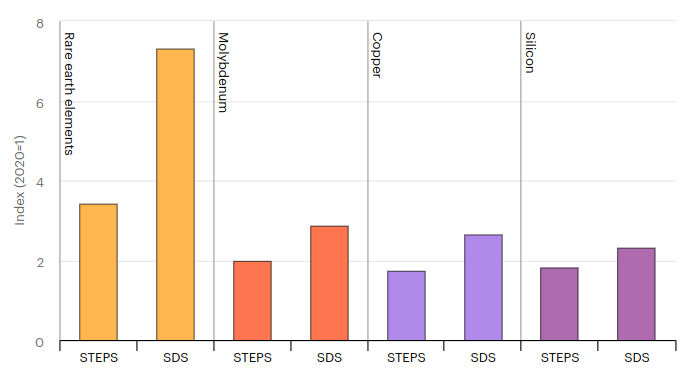
\includegraphics[width=\textwidth]{130quantification/external/energy_change_demand.png}
    \caption{Change in demand for selected elements}\label{fig:energy_change_demand}
\end{figure}

\begin{figure}[h!]
    \centering
    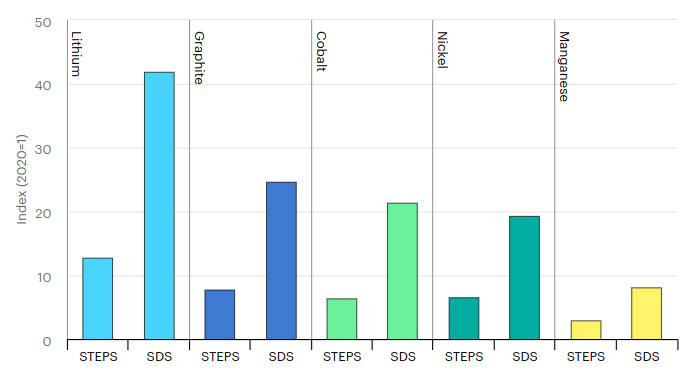
\includegraphics[width=\textwidth]{130quantification/external/energy_change_batt_demand.png}
    \caption{Change in demand for battery relevant elements}\label{fig:energy_demand_batt}
\end{figure}

\begin{figure}[h!]
    \centering
    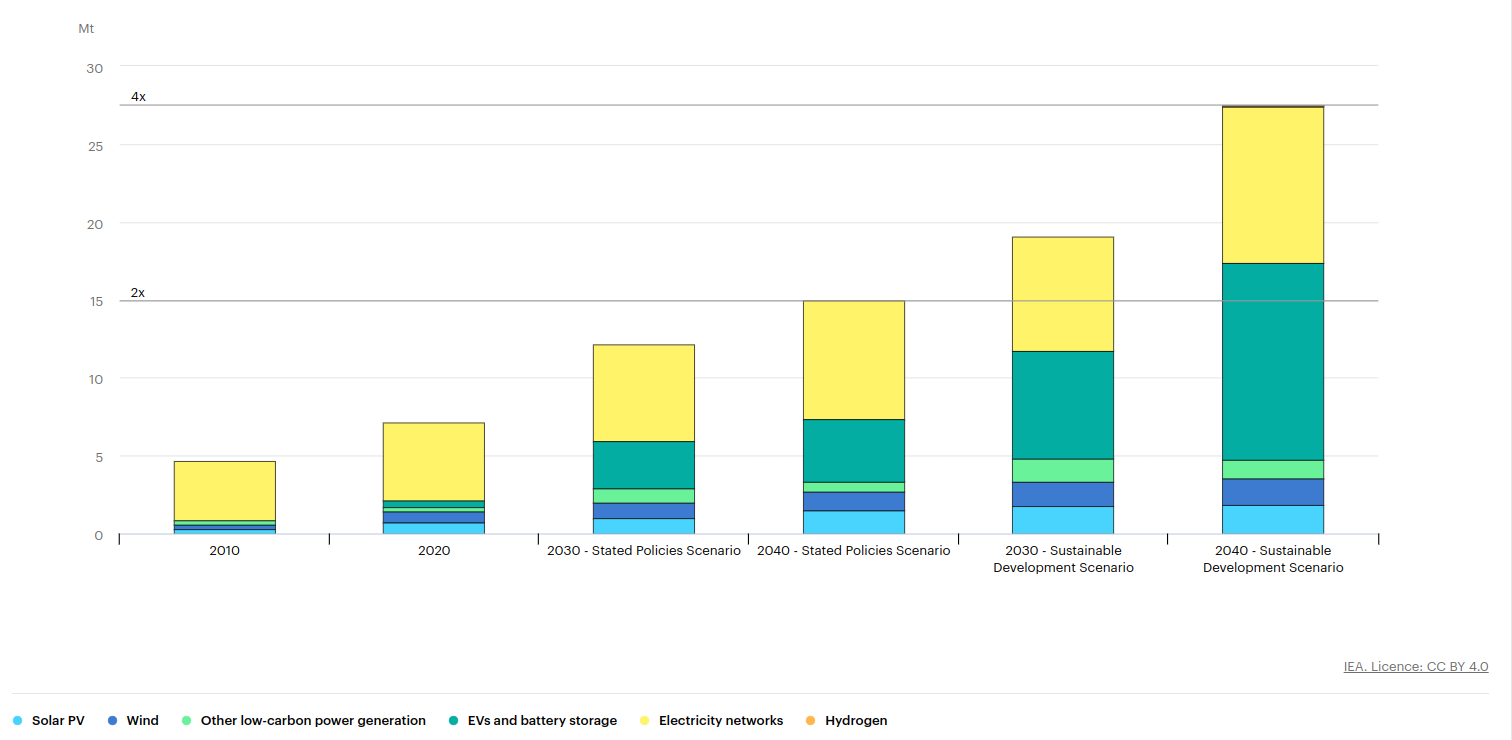
\includegraphics[width=\textwidth]{130quantification/external/energy_total_demand.png}
    \caption{Global mineral demand (total) under various scenarios}\label{fig:energy_mineral_total}
\end{figure}

\subsectionEndline
\clearpage

\subsubsection{Incorporation of the energy transition into individual waste stream models}


\boxws{This section will be filled out with the details of exactly how this parameter is incorporated into your stock and flow models}


\wasteSubsubsubsecBATT
\vspace{-1cm}
\begin{itemize}
    \item X
\end{itemize}

\wasteSubsubsubsecCDW
\vspace{-1cm}
\begin{itemize}
    \item X
\end{itemize}

\wasteSubsubsubsecELV
\vspace{-1cm}
\begin{itemize}
    \item X
\end{itemize}

\wasteSubsubsubsecMIN
\vspace{-1cm}
\begin{itemize}
    \item X
\end{itemize}

\wasteSubsubsubsecSLASH
\vspace{-1cm}
\begin{itemize}
    \item X
\end{itemize}

\wasteSubsubsubsecWEEE
\vspace{-1cm}
\begin{itemize}
    \item X
\end{itemize}



\subsectionEndline

\clearpage
